

\section{Experimental setup and data samples}
\label{sec:experiment}

%Data Samples
The analysis is based on pp and p--Pb data collected during the LHC Run 2 period. The pp collisions had a center of mass energy $\sqrt{s} = 13$ TeV, and they were recorded from 2016 to 2018.
The p–-Pb collisions had a center of mass energy per nucleon-nucleon pair $\sqrt{s_\mathrm{NN}} = 5.02$~TeV, and they were collected in 2016. It is worth noting that there is a shift in the center-of-mass rapidity of $\Delta y$ = 0.465 in the direction of the proton beam due to the asymmetric collision system.

%Basic description of detectors
A comprehensive description of the ALICE detector and its performance can be found in Refs.~\cite{Aamodt:2008zz, Abelev:2014ffa, ALICE:2022wpn}. The analysis utilizes the V0 detector~\cite{Abbas:2013taa}, the Inner Tracking System (ITS)~\cite{aliceITS, ALICE:2013nwm}, and the Time Projection Chamber (TPC)~\cite{aliceTPC}. 

The V0 detector consists of two stations on both sides of the interaction point, V0A and V0C, each comprising of 32 plastic scintillator tiles, covering the full azimuthal angle within the pseudorapidity intervals $2.8 < \eta < 5.1$ and $-3.7 < \eta < -1.7$, respectively. 
The ITS is a silicon tracker with six layers of silicon sensors. The two innermost layers of the ITS are called the Silicon Pixel Detector (SPD)~\cite{Santoro2009:ALICESPD}. In addition to the two SPD layers, the middle two layers are the SDD (Silicon Drift Detector), and the outermost layers are the SSD (Silicon Strip Detector). The TPC is a gas-filled cylindrical tracking detector providing up to 159 reconstruction points for charged tracks traversing the full radial extent of the detector.

%Usage of detectors: triggers, PV, tracking etc
The V0 provides a minimum bias (MB) trigger in both pp and p--Pb collisions and an additional high-multiplicity trigger in pp collisions. The MB trigger is obtained by a time coincidence of V0A and V0C signals. 
Amplitudes of V0A and V0C signals are proportional to charged-particle multiplicity, and their sum is denoted as V0M.  
The high-multiplicity trigger in pp collisions requires the V0M signal to exceed five times the mean value measured in MB collisions, selecting the 0.1\% of MB events with the largest V0M multiplicity. The centrality in p--Pb collisions is determined using the V0A detector, which is located in the Pb-going direction. The analyzed data samples of MB and high-multiplicity pp events at $\sqrt{s}=$~13 TeV correspond to integrated luminosities ($\mathcal{L}_\mathrm{int}$) of about 19 nb$^{-1}$ and 11 pb$^{-1}$, respectively~\cite{ALICE:2016nst}. In p--Pb collisions at $\sqrt{s_\mathrm{NN}} = 5.02$ TeV, the corresponding integrated luminosity is $\mathcal{L}_\mathrm{int} \sim 0.3$ nb$^{-1}$. 

Positions of primary vertices are reconstructed from signals measured by the SPD. The reconstructed primary vertices are required to be within 8 cm of the nominal interaction point along the beam direction. 
Pileup events are identified as events with multiple reconstructed primary vertices. These events are rejected if the distance between any of the vertices to the main primary vertex is greater than 0.8 cm.
The probability of pileup events is estimated to range from $10^-3$ to $10^-2$ for MB and high-multiplicity events in pp collisions~\cite{ALICE:2020swj}. The pileup probability is estimated to be negligible in p--Pb collisions~\cite{ALICE:2017svf}. 

Charged-particle tracks are reconstructed using the combined information from the ITS and TPC.
%Charged-particle tracks are reconstructed using the combined information of the ITS and TPC in a uniform magnetic field of 0.5 T along the beam direction provided by the L3 solenoidal magnet. 
For charged particles emitted from a vertex located within $|z_\mathrm{vtx}|<8$ cm along the beam direction, the ITS and TPC provide a pseudorapidity coverage of $|\eta|<1.4$ and 0.9, respectively. Both detectors have full coverage in azimuth. They are placed in a uniform magnetic field of 0.5 T that is oriented along the beam direction.

The charged-particle-selection criteria are optimized to ensure a uniform efficiency over the midrapidity range $|\eta|<0.9$ to mitigate the effects of small areas where some ITS layers are inactive in both collision systems. The selected sample of tracks consists of two classes. Tracks in the first class must have at least one hit in the SPD. Tracks of the second class do not have any hits in the SPD, but their origin is constrained to the primary vertex~\cite{ALICE:2012eyl}. 
Charged-particle tracks are reconstructed down to a transverse momentum ($\pt$) of 0.15 GeV/$c$ with an efficiency of approximately 65\%~\cite{Ivanov:2006yra}. The efficiency increases to 80\% for particles with $\pt>1$ GeV/$c$. The $\pt$ resolution is approximately 1\% for primary charged particles~\cite{ALICE-PUBLIC-2017-005} with $\pt<$ 1~GeV/$c$, and it linearly increases to 6\% at $\pt\sim$ 50~GeV/$c$ in pp collisions and 10\% in p--Pb collisions~\cite{ALICE:2018vuu}.


\section{Analysis procedure}
\label{sec:ana}
\subsection{Two-particle angular correlations}
Two-particle angular correlations are measured as a function of the relative azimuthal angle ($\Delta\varphi$) and the relative pseudorapidity ($\Delta\eta$) between a trigger and associated particles
\begin{eqnarray}
\frac{1}{N_{\rm{trig}}} \frac{ \rm{d}\it{}^{2} N_{\rm{pair}} }{ \rm{d} \Delta\eta \rm{d}\Delta\varphi} = B(0, 0)\frac{S(\Delta\eta, \Delta\varphi)}{B(\Delta\eta, \Delta\varphi)}  \Big\lvert_{\pttrig,\,\ptassoc},
\label{eq:corrfunction}
\end{eqnarray}
where $p_\mathrm{T,trig}$ and $p_\mathrm{T,assoc}$ denote the transverse momentum of the trigger and associated particles, respectively.
While the transverse momentum range for associated particles is fixed to $1<p_\mathrm{T,assoc}<4$~GeV/$c$ for trigger particles, several transverse momentum ranges are considered. The lower limit of $p_\mathrm{T,trig}$ and $p_\mathrm{T,assoc}$ ($>$~1~GeV/$c$) is chosen in order to avoid jet-like contributions from lower $p_\mathrm{T}$ particles which extend into the larger $\Delta\eta$ range because of the limited $\eta$ acceptance~\cite{ALICE:2021nir}. The numbers of trigger particles and trigger--associated particle pairs are denoted as $N_\mathrm{trig}$ and $N_\mathrm{pair}$, respectively.
The quantity $S(\Delta\eta, \Delta\varphi)$ represents the average number of pairs in the same event, while $B(\Delta\eta, \Delta\varphi)$ denotes the number of pairs obtained by the event mixing technique. The normalization of $B(\Delta\eta, \Delta\varphi)$ is represented by $B(0,0)$. To correct for acceptance effects, $S(\Delta\eta, \Delta\varphi)$ is divided by $B(\Delta\eta, \Delta\varphi)/B(0,0)$. The particles are weighted by the inverse of the tracking efficiency, which is obtained in the same way as in a previous study~\cite{ALICE:2021nir}. In that study, the tracking efficiency was calculated using a detector simulation with the PYTHIA 8 event generator and the GEANT3 transport code~\cite{Brun:1994aa}. To account for differences in particle composition between real data and PYTHIA, the tracking efficiency is determined from a PYTHIA-based simulation with re-weighted primary particle-species composition.
The weights reflect realistic abundances of different particle species, which were extracted by a data-driven method~\cite{ALICE:2018hza, ALICE:2018vuu}.
%Therefore, this method improves the jet-yield extraction and has no impact on the flow extraction.
Events to be mixed are required to have primary vertices within the same 2 cm wide $z_{\rm vtx}$ interval. The correlation functions are averaged over the vertex intervals, resulting in the final per-trigger yield~\cite{Kopylov:1974th,Adam:2016tsv}. 

\begin{figure}[h!]
		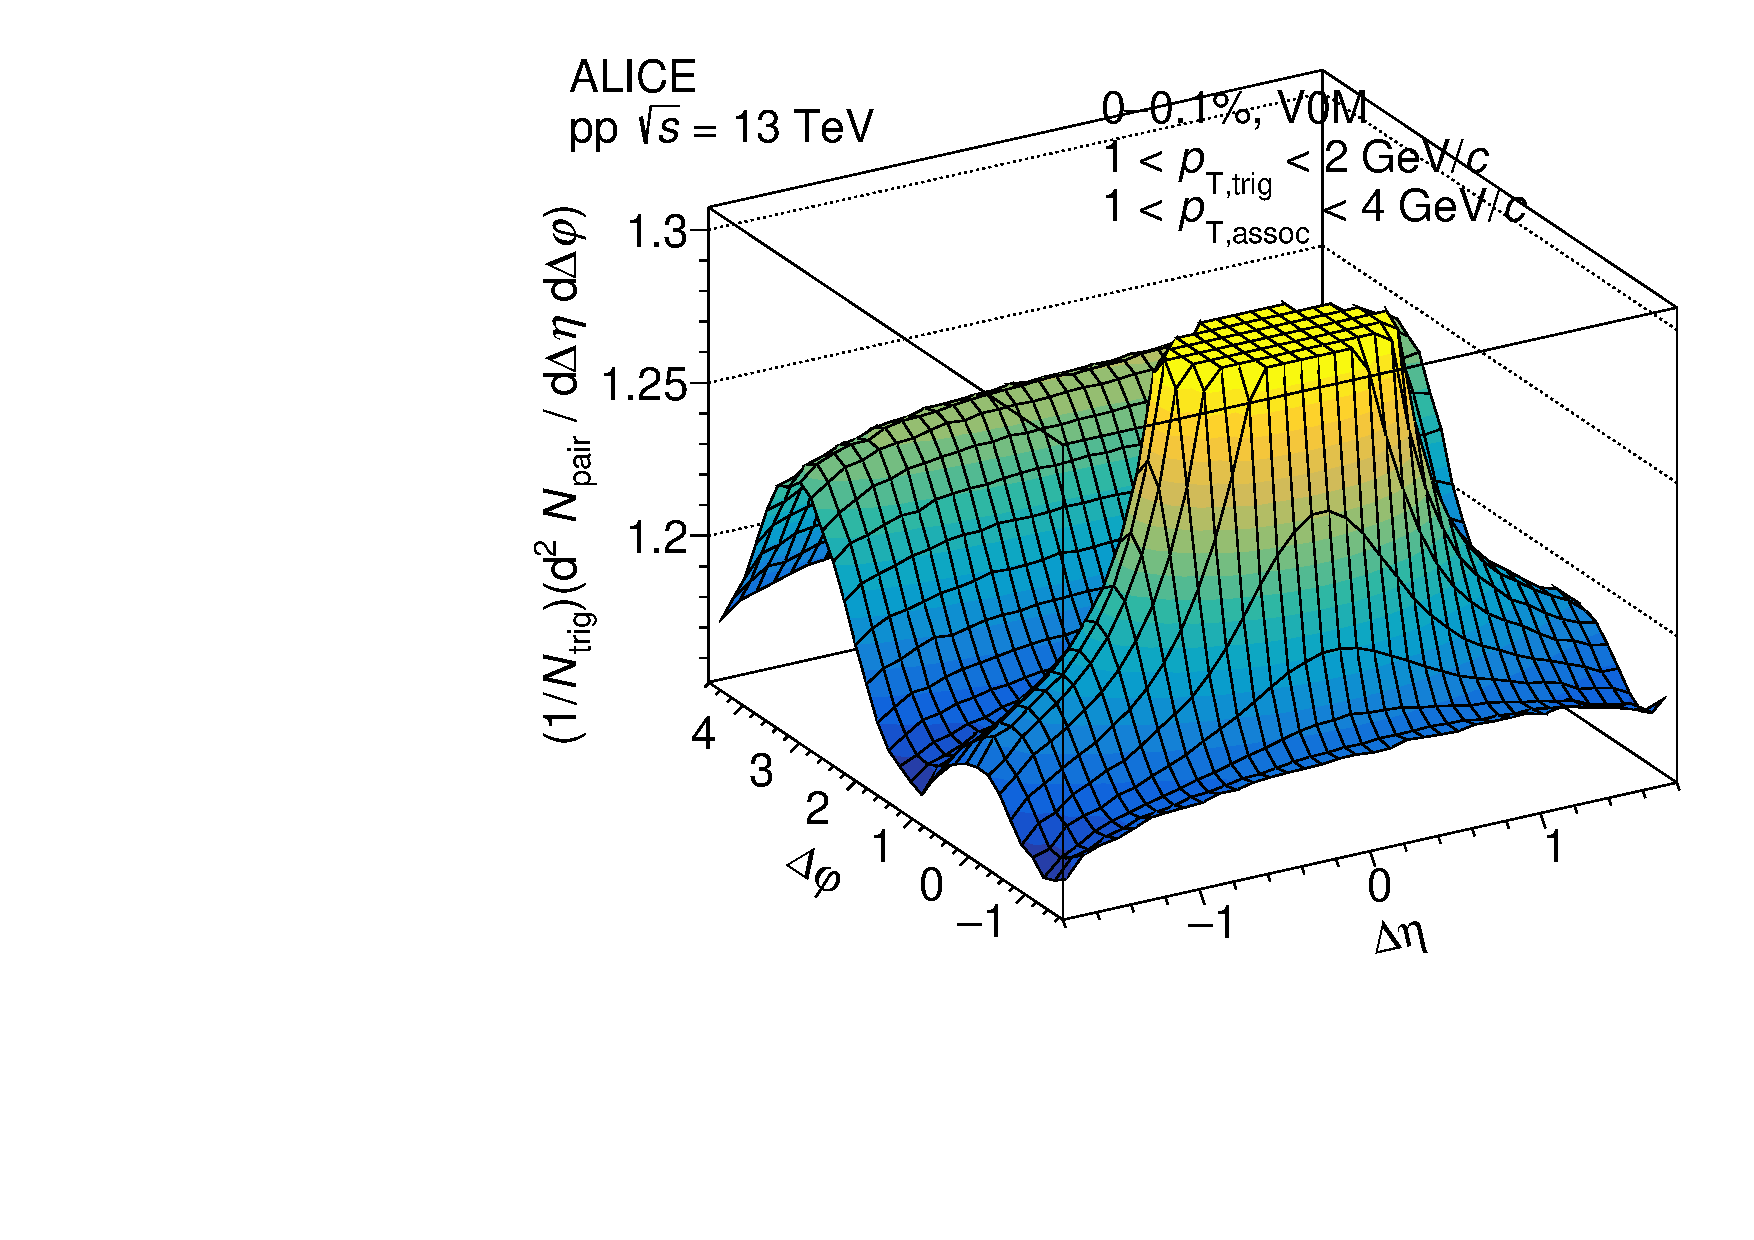
\includegraphics[width=0.5 \textwidth]{figures/FIG1_ppHigh.pdf} 
		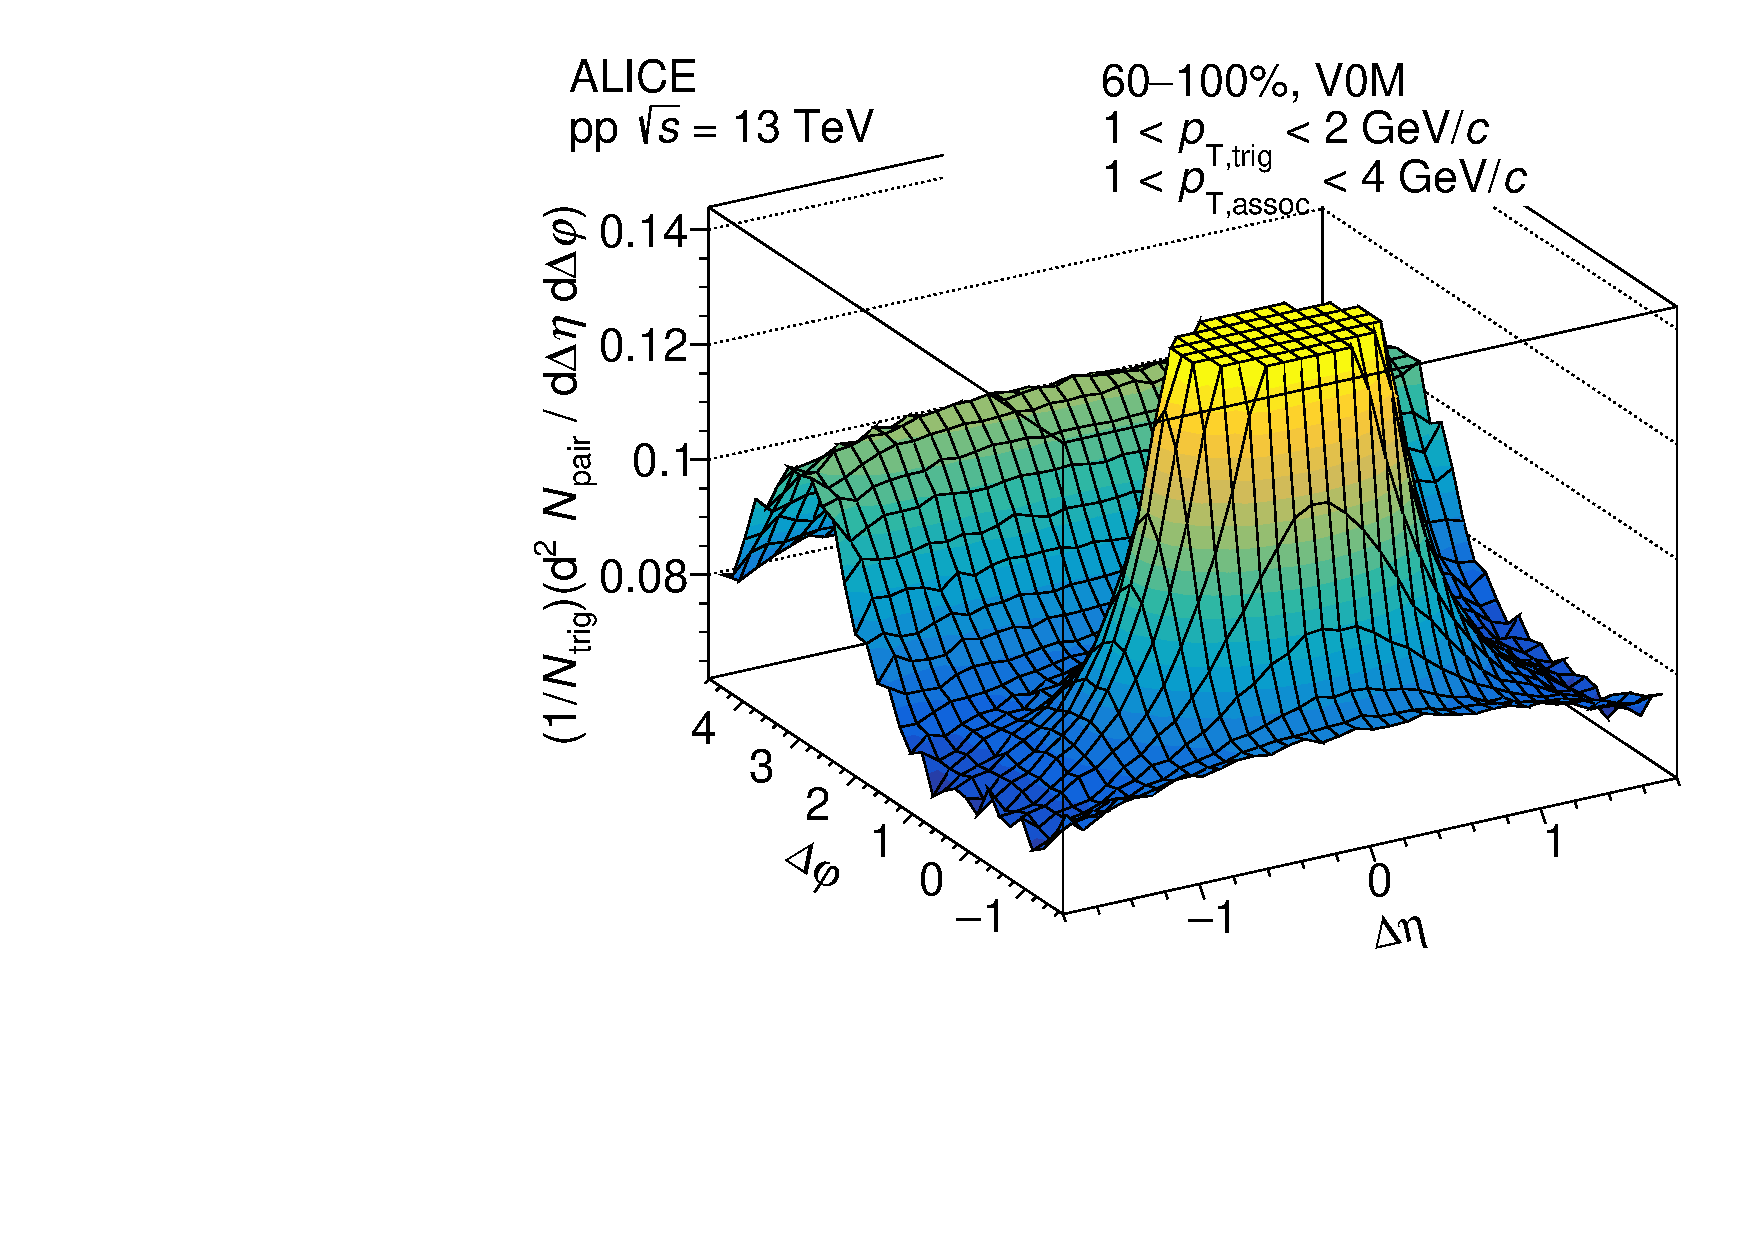
\includegraphics[width=0.5 \textwidth]{figures/FIG1_ppLow.pdf} 
  		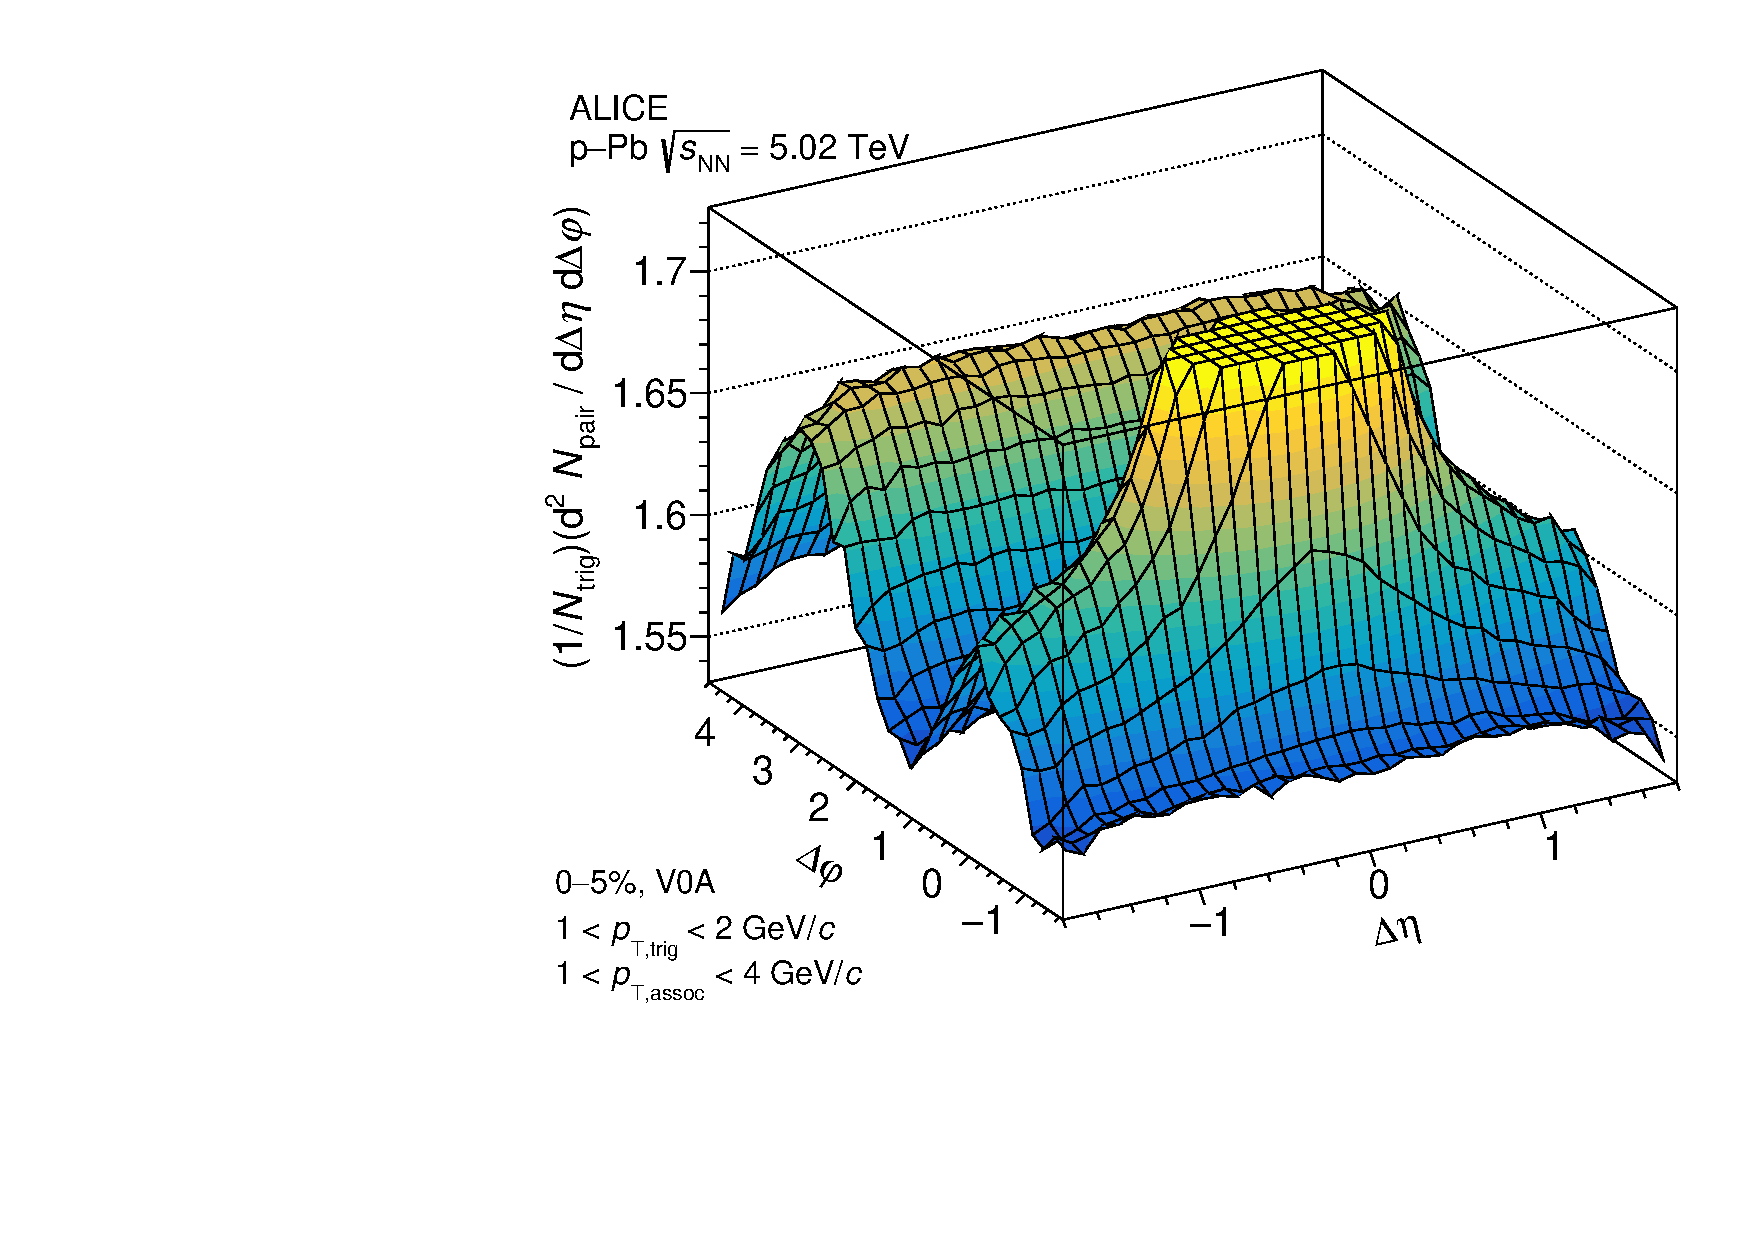
\includegraphics[width=0.5 \textwidth]{figures/FIG1_pPbHigh.pdf}
		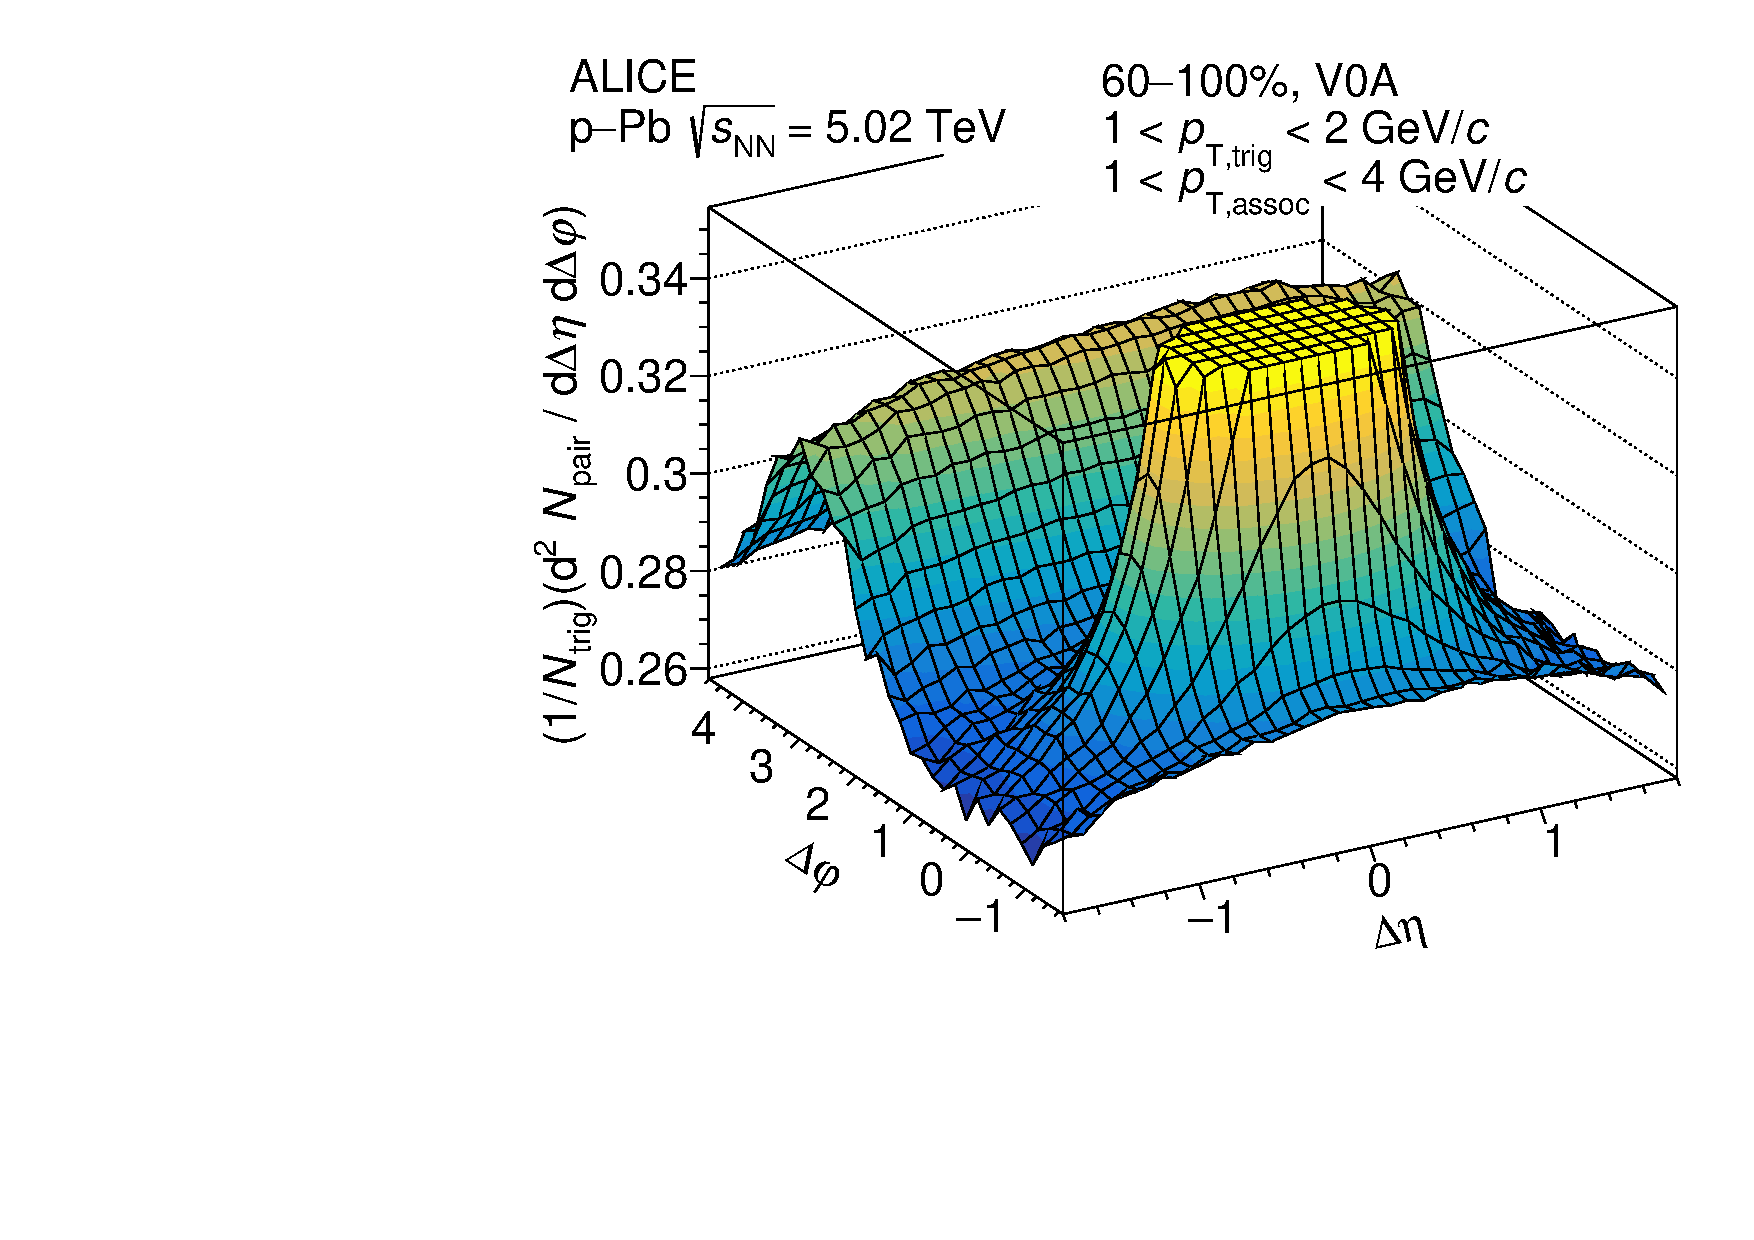
\includegraphics[width=0.5 \textwidth]{figures/FIG1_pPbLow.pdf}
\caption{Two-dimensional correlation functions are presented for high-multiplicity (0--0.1\% or 0--5\%, on the left) and low-multiplicity (60--100\%, on the right) events in $\sqrt{s}=13$ TeV pp collisions in the top panels. The corresponding distributions for $\sqrt{s_{\mathrm{NN}}}=5.02$ TeV p--Pb collisions are shown in the bottom panels. All correlation functions are shown for 1~$<\it{p}_{\rm{T,trig}}<$~2~GeV/$c$ and 1~$<\it{p}_{\rm{T,assoc}}<$~4~GeV/$c$, respectively.}
\label{fig:doubleridge}
\end{figure}

The fully corrected correlation functions from pp and p--Pb collisions are shown in Fig.~\ref{fig:doubleridge}. 
The $z$-axis is scaled in order to exhibit the ridge structures at large $\Delta\eta$ regions. As a result, the jet peaks are sheared off in all figures. The flow modulation structure is clearly observed to emerge in the high-multiplicity collisions for both systems, while it is not seen in the low-multiplicity collisions. The away-side regions are populated mostly by back-to-back jet correlations. 

The per-trigger yield is determined by integrating the correlation function at large $\Delta\eta$ ($1.6<|\Delta\eta|<1.8$) to remove non-flow contributions from near-side jet fragments.
The per-trigger yield as a function of $\Delta\varphi$ is expressed as

\begin{eqnarray}
Y(\Delta\varphi) = \frac{1}{N_{\mathrm{trig}}} \frac{\mathrm{d} N_{\mathrm{pair}}}{\mathrm{d}\Delta\varphi} = \int_{1.6<|\Delta \eta|<1.8} \left[\frac{1}{N_{\mathrm{trig}}} \frac{\mathrm{d}^{2}N_{\mathrm{pair}}}{\mathrm{d}\Delta\eta \mathrm{d}\Delta\varphi}\right] \frac{1}{\delta_{\Delta\eta}} \mathrm{d}\Delta \eta,
\label{eq:pertrigger}
\end{eqnarray}

where the factor $\delta_{\Delta\eta}=$~0.4 normalizes the obtained per-trigger yield per unit of pseudorapidity.
The per-trigger yields are extracted for the considered $p_{\mathrm{T,trig}}$ and $/p_{\mathrm{T,assoc}}$ intervals in several multiplicity classes: 0--0.1\%, 1--5\%, 5--20\%, 20--60\%, and 60--100\% in pp collisions, and 0--5\%, 5--10\%, 10--20\%, 20--40\%, 40--60\%, and 60--100\% in p--Pb collisions. The conversion of the measured forward event multiplicities to the multiplicities in the midrapidity ($N_{ch}$ ($|\eta|<0.5$)) used in Sec.~\ref{sec:results} is based on Refs.~\cite{ALICE:2020swj}.

\subsection{Extraction of flow coefficients}

As discussed in Refs.\cite{ATLAS:2015hzw,ATLAS:2016yzd}, the correlation function in a given multiplicity interval is fitted with 
\begin{eqnarray}
\label{eq:narray}
Y_{\rm{HM}}(\Delta\varphi) = G~(1 + 2v_{2,2}\cos(2\Delta\varphi) + 2v_{3,3}\cos(3\Delta\varphi)) + F~Y_{\rm{LM}}(\Delta\varphi),
\label{eq:tmpfit}
\end{eqnarray}
where $Y_{\rm{LM}}(\Delta\varphi)$ is the measured per trigger yield from low-multiplicity events. The normalization factor for the first three Fourier terms, which parameterize the long-range, flow-like, correlation is denoted as $G$. The scale factor $F$ compensates for the increased yield of away-side-jet hadrons in the analyzed multiplicity class relative to the low-multiplicity template that corresponds to the 60--100\% class~\cite{ALICE:2013tla,ALICE:2014mas}.
The fit determines the scale factor $F$, pedestal $G$, and $v_{n,n}$ and is performed in various high-multiplicity classes as well as in different $p_\mathrm{T,trig}$ and $p_\mathrm{T,assoc}$ intervals. 
This method assumes that $Y_{\rm{LM}}$ does not contain a near-side-peak structure that would originate from jet fragmentation or near-side ridge.
Further it is assumed that the shape of the away-side-peak structure remains the same when changing multiplicity class.
The first assumption is ensured using the selected low-multiplicity template which doesn't have a strong near-side-peak structure compared to the studied higher multiplicity classes. The second assumption, which involves the modification of jet shapes, was tested by projecting the near-side jet peaks onto $\Delta\eta$. This projection did not reveal any strong dependence of the jet-peak shape on multiplicity class~\cite{LAKOMOV2017329}. However, the effect of the possible modification of the away-side jet yield on the result of the template fit was investigated by adjusting the away-side shape based on the observed differences between low- and high-multiplicity events. The effect on the extracted $v_2$ was found to be less than 1$\%$ in pp and p--Pb collisions for the kinematic selections used in this analysis. As for $v_3$, the maximum effect is about 3\% and 8$\%$ in pp and p--Pb collisions, respectively.  This modification of the jet shape is considered as one of the sources of systematic uncertainty and will be discussed in Sec.~\ref{sec:uncertainties}.

\begin{figure}[h!]
	\centering
	\hspace{-3em}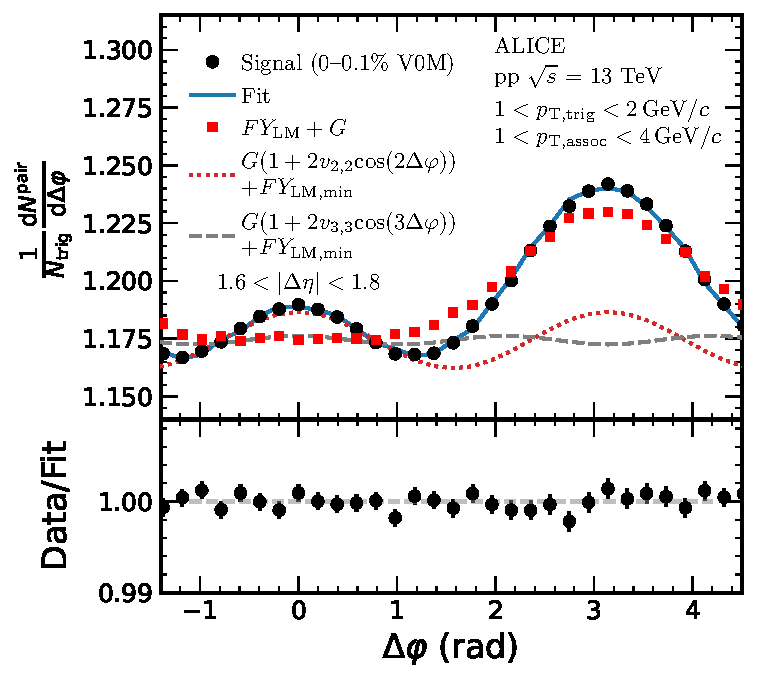
\includegraphics[width=0.6\textwidth]{figures/FIG2_FlowExt.pdf} 
	\caption{Per-trigger yield in $1.6<|\Delta\eta|<1.8$ extracted from 0--0.1\% and 60--100\% multiplicity percentile events in $\sqrt{s}=13$ TeV pp collisions. The data are fitted with the template fit method described by Eq.~\ref{eq:tmpfit}. The black markers show the signal for the 0--0.1\% multiplicity percentile. The red squares correspond to the low-multiplicity signal. The red and gray curves correspond to the extracted $v_{2,2}$ and $v_{3,3}$ signals, respectively. To improve visibility, the baselines of flow signals are scaled by $FY_{\mathrm{LM,min}}$, which represents the minimum yield of $FY(\Delta\varphi)_{\mathrm{LM}}$. The signal-to-fit ratio is shown in the bottom panel. The $\chi^{2}$ divided by the number of degrees of freedom is 0.894.}
	\label{fig:flowext}
\end{figure}

Figure~\ref{fig:flowext} shows the template fit results for the 0--0.1\% multiplicity interval in pp collisions at $\sqrt{s} = $13~TeV. Values of the extracted scale factor $F$ in different multiplicity intervals and systems are summarized in Table~\ref{tab:FpppPb}. In pp collisions, the value of $F$ is observed to increase slightly as the event multiplicity increases. The F value, which is measured for the highest multiplicity bin, is approximately 25\% larger than the value found for the 20–60\% bin. A similar dependence on multiplicity is observed for p--Pb collisions, although the dependence on the multiplicity interval is weaker. When comparing F values from pp and p–Pb collisions which have similar centrality, the value of $F$ in p--Pb collisions is found to be smaller and closer to unity.
This suggests that the jet fragmentation yield on the away-side increases with multiplicity, and that this feature is more pronounced in pp collisions. The difference between the two systems is likely to be explained by the true-geometry-driven centrality in p--Pb collisions, as opposed to the jet-dominated bias in pp collisions.
The previous analyses published by ALICE in Refs. ~\cite{ALICE:2012eyl,ALICE:2013snk} assumed that the jet contribution remains constant as a function of multiplicity (i.e. $F$ was assumed to be 1). However, this assumption may lead to an underestimation of non-flow contamination in the measurements of anisotropic flow.

\begin{table}[!b]
\caption{The scale factor $F$ for various multiplicity intervals is shown for pp collisions (top) and p--Pb collisions (bottom), with 1~$<\it{p}{\rm{T,trig}}<$~2~GeV/$c$ and 1~$<\it{p}{\rm{T,assoc}}<$~4~GeV/$c$. Note that only statistical uncertainties are reported in the table. The systematic uncertainty for $F$ is 3.8\%, which is the same for both collision systems and multiplicity intervals.}
\centering
\resizebox{\textwidth}{!}{%
\begin{tabular}{|c|c|c|c|c|c|c|}
\hline
	V0M (pp)& 0--0.1\% & 1--5\% & 5--20\% & 20--60\% & &\\
\hline
	$F$ & 1.504$\pm$0.017 & 1.414$\pm$0.030 & 1.360$\pm$0.019 & 1.208$\pm$0.015 & & \\
\hline
V0A (p--Pb)& 0--5\% & 5--10\% & 10--20\% & 0--20\% & 20--40\% & 40--60\% \\
\hline
$F$& 1.135$\pm$0.026 & 1.140$\pm$0.026 & 1.152$\pm$0.021 & 1.145$\pm$0.017 &1.092$\pm$0.015 & 1.083$\pm$0.015 \\
\hline
\end{tabular}
}
\label{tab:FpppPb}
\end{table}

In the following, the near and away-side jet fragmentation yields are calculated to verify the template fit method by comparing the jet fragmentation yields to the PYTHIA model. The away-side jet fragmentation yields in the PYTHIA model are obtained using the standard $\Delta\varphi$ analysis, while the away-side jet fragmentation yields are extracted using the template fit method due to the flow modulations in the data. The comparison between the data and the PYTHIA model provides a validation of the template fit method. 

Equivalently to Eq.~\eqref{eq:pertrigger}, the near-side $\Delta\eta$ correlations are obtained with
\begin{equation}
Y(\Delta\eta)=\frac{1}{N_{\rm{trig}}} \frac{ \rm{d}\it{}N_{\rm{pair}} }{ \rm{d}\Delta\eta }=\int_{|\Delta\varphi|<1.3}\left[ \frac{1}{\it{N}_{\rm{trig}}} \frac{ \rm{d}\it{}^{2} N_{\rm{pair}} }{ \rm{d}\Delta\eta d\Delta\varphi} \right]\dfrac{1}{\delta_{\Delta\varphi}} {\rm{d}}\Delta \varphi - D_\mathrm{ZYAM},
\label{eq:deltaetacorr}
\end{equation}
where $\delta_{\Delta\varphi}=2.6$. Additionally, $D_\mathrm{ZYAM}$ defines the baseline of the ZYAM background subtraction~\cite{Ajitanand:2005jj}, obtained by minimizing the first term on the right-hand side within $|\Delta\eta|<1.6$. Due to the shape of the correlation function the minimum is found at $|\Delta\eta|=1.3$.
The near-side jet-like yields were extracted by integrating the $Y(\Delta\eta)$, which can be expressed as
\begin{eqnarray}
Y^\mathrm{near}_{\rm{frag}} = \int_{|\Delta \eta|<1.3} \left( \frac{1}{\it{N}_{\rm{trig}}} \frac{ \rm{d}\it{}N_{\rm{pair}} }{ \rm{d}\Delta\eta } \right) \rm{d} \Delta\eta.
\label{eq:Ynear}
\end{eqnarray}

As flow has a weak $\eta$ dependence~\cite{ATLAS:2011ah,PHENIX:2018hho,ALICE:2016tlx}, the jet-fragmentation yield can be calculated after the ZYAM background subtraction~\cite{Ajitanand:2005jj}. 
The away-side jet-like yield in data is calculated by integrating the low-multiplicity template over $\pi/2<\Delta\varphi<3/2\pi$ and scaling it by the parameter $F$ from Eq.~\ref{eq:narray}, $Y^{\rm{away, HM}}_{\mathrm{frag}} = Y^{\rm{away, LM}}_{\mathrm{frag}} \times F$. The $Y^{\rm{away, LM}}_{\mathrm{frag}}$ is directly obtained by integrating the away-side low-multiplicity $\Delta\varphi$ correlation function in the low-multiplicity sample over $\pi/2 < \Delta\varphi < 3\pi/2$.
While PYTHIA does not include any flow contributions in its model, $Y^{\rm{away}}$ can be directly measured from the $\Delta\varphi$ correlation functions.

\begin{figure}[h!]
	\centering
	\hspace{-3em}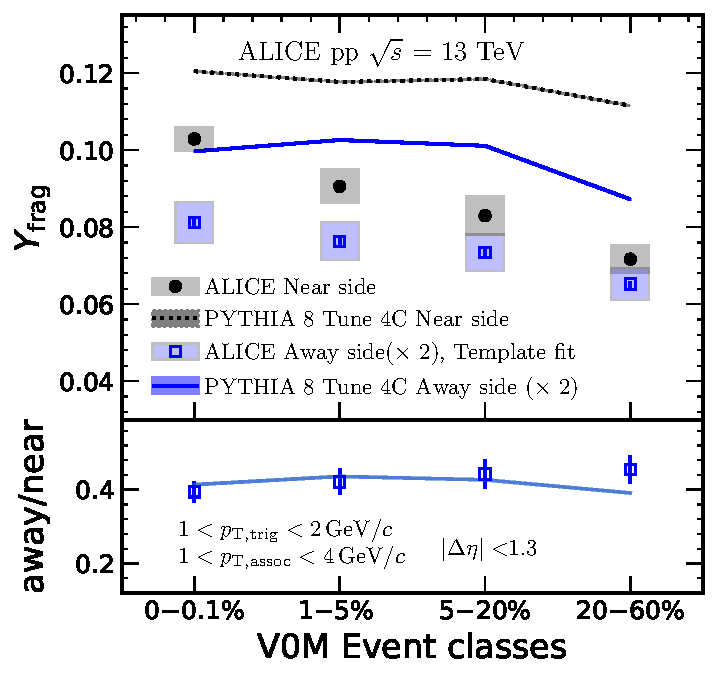
\includegraphics[width=0.6\textwidth]{figures/FIG3_Plot_v2Mult.pdf} 
	\caption{The $Y_{\rm{frag}}$ for the near- and away-side as a function of multiplicity percentiles with both ALICE and PYTHIA data. The boxes around the data points in the top panel describes the systematic uncertainty estimation of each data point. The ratio includes the combined statistical and systematic errors added in quadrature. ALICE measurements are shown as circle and square markers, whereas PYTHIA is shown as lines. The near-side yields are shown in black, and the away-side yields in blue.}
	\label{fig:Ymult}
\end{figure}

Figure~\ref{fig:Ymult} presents the $Y^{\mathrm{near}}_{\rm{frag}}$ and $Y^{\mathrm{away}}_{\rm{frag}}$, for both ALICE data and PYTHIA 8 Tune 4C~\cite{Skands:2014pea}, as a function of the V0M multiplicity percentile in pp collisions at $\sqrt{s}=13$ TeV. The transverse momentum range for trigger particles is $1<p_\mathrm{T,trig}<2$ GeV/$c$ and for associated particles $1<p_\mathrm{T,assoc}<4$ GeV/$c$.
The near- to away-side ratio for ALICE and PYTHIA data is shown in the bottom panel. While PYTHIA overestimates both near-side and away-side yields measured by ALICE, the ratio in PYTHIA is consistent with the ALICE data in the all considered V0M multiplicity intervals. The value of this ratio can be explained by the pair acceptance effect caused by the limited ALICE $\eta$ acceptance~\cite{PHENIX:2006gto}, which implies that the enhanced jet fragmentation yields in the away-side in high-multiplicity events with respect to low-multiplicity events~\cite{ALICE:2013tla,ALICE:2014mas} are taken into account by the low-multiplicity template method. In summary, the difference between the near-side and away-side jet fragmentation yields in PYTHIA is solely caused by the jet acceptance effects of the two-particle correlation functions. This ratio in data where the away-side jet fragmentation yields are measured with the low-multiplicity template agrees well with PYTHIA as well as the calculations in Ref.~\cite{PHENIX:2006gto}.

The flow coefficients, $v_{n}$, of the trigger particles, can be extracted from the template fit with the use of the observed factorization of $v_{n,n}$ coefficients to single harmonics~\cite{ATLAS:2015hzw,ATLAS:2016yzd} by using
\begin{eqnarray}
v_{n}(p_{\rm{T,trig}}) = v_{n,n}(p_{\rm{T,trig}}, p_{\rm{T,assoc}}) / \sqrt{ v_{n,n}(p_{\rm{T,assoc}},p_{\rm{T,assoc}})},
\end{eqnarray}
where $v_{n,n}(p_{\rm{T,assoc}}, p_{\rm{T,assoc}})$ are measured in 1~$<p_{\rm{T,trig}}<$~4~GeV/$c$ interval as the $p_{\rm{T,assoc}}$ range is fixed with 1~$<p_{\rm{T,assoc}}<$~4~GeV/$c$. In the following sections, unless explicitly stated otherwise, $v_n$ will refer to $v_n(p_{\rm{T,trig}})$.
Different event scale selections were investigated by selecting events that include a hard jet or a high-$\pt$ leading particle in midrapidity (i.e., the highest reconstructed $\pt$ inside the acceptance region in an event).
This event scale was set by requiring a minimum $\pt$ of the leading track ($\ptlead$) or the reconstructed jet ($\ptjet$) at midrapidity~\cite{ALICE:2021nir}. The leading particle track was required to be within $|\eta|<0.9$ and $0<\varphi<2\pi$, and the jets were reconstructed with the anti-$k_{\rm{T}}$ algorithm~\cite{Cacciari:2008gp,Cacciari:2011ma}, with $R=0.4$ using charged particles only. Jet constituents were combined using the boost-invariant $\pt$ recombination scheme. The jets are selected in the full azimuth ($0<\varphi<2\pi$)and their pseudorapidity is constrained to $|\eta_\mathrm{jet}|<0.4$. The $\pt$ of jets $\ptjet$ is corrected for the underlying event density that is measured using the $k_{\rm{T}}$ algorithm with $R=$~0.2 following the procedure described in Ref.~\cite{Acharya:2018eat}.

%%%%%%%%%%%%%%%%%%%%%%%%%%%%%%%%%%%%%%%%%%%%%%%%%%%%%%%%%%

\section{Systematic uncertainties}
\label{sec:uncertainties}

\begin{table}[h!]
\caption{The relative systematic uncertainties of $Y^{\rm{near}}$, $Y^{\rm{away,LM}}$, $F$, $v_{2}$, and $v_{3}$. $Y^{\rm{near}}$, $Y^{\rm{away,LM}}$, $F$, are only measured in pp collisions, whereas $v_{2}$, and $v_{3}$ are measured in both pp and p--Pb collisions. The quoted ranges correspond to minimum and maximum uncertainties. Those uncertainties that are considered to be negligible are marked ``negl.". The systematic variations which are not relevant for the measurement are denoted as ``N.A".}
\centering
\label{tab:syst}
\resizebox{\textwidth}{!} {
\begin{tabular}{c|ccc|cccc}
\hline 
\multirow{3}{*}{Sources}  & \multicolumn{7}{c}{Systematic uncertainty (\%)} \\ \cline{2-8} 
& \multicolumn{1}{c}{$Y^{\rm{near}}$} & \multicolumn{1}{c}{$Y^{\rm{away,LM}}$} & \multicolumn{1}{c|}{$F$} & \multicolumn{2}{c}{$v_{2}$} & \multicolumn{2}{c}{$v_{3}$}  \\  \cline{2-8}
&pp &pp &pp & pp & p--Pb & pp & p--Pb  \\ \cline{1-8} 
Primary vertex       & $\pm$0.2--0.5 & $\pm$0.1      & $\pm$1.0--2.5 & $\pm$0.2--1.8 & $\pm$0.8 & $\pm$1.4 & $\pm$3.9 \\ 
Pileup rejection     & $\pm$0.1--0.5 & $\pm$0.2      & $\pm$0.4--1.5 & negl.         & $\pm$0.6 & negl. & $\pm$1.4 \\ 
Tracking		     & $\pm$1.0--3.0 & $\pm$2.0      & $\pm$0.6--2.4 & $\pm$0.2--3.0 & negl. & $\pm$5.0--6.9 & negl. \\ 
Event mixing	     & $\pm$0.2--0.7 & $\pm$0.2--0.5 & $\pm$0.0--3.3 & $\pm$0.3--4.6 & $\pm$0.8 & $\pm$2.8--3.1 & $\pm$0.8 \\ 
Low-mult. definition & N.A.          & $\pm$0.5--3.5 & $\pm$0.7--6.0 & negl.         & $\pm$1.9 & negl. & $\pm$9.2\\ 
ITS--TPC matching 	 & $\pm$2.0--3.0 & $\pm$2.0--3.0 & N.A.          & N.A.          & N.A. & N.A. & N.A\\ 
Efficiency correction& $\pm$1.0--4.4 & $\pm$1.0--4.4 & N.A.          & N.A.          & N.A. & N.A. & N.A\\ 
$\Delta\eta$ gap range   	 & N.A.          & N.A.          & $\pm$0.1--3.2 & $\pm$1.0--5.0 & $\pm$0.4 & negl. & negl. \\ 
Jet shape modification   	 & N.A.          & N.A.          & N.A &  $\pm$1.0& $\pm$1.0 & $\pm$3.0 & $\pm$8.0 \\ 
\hline 
Total (in quadrature)& $\pm$2.5--6.1 & $\pm$5.0--5.5 & $\pm$1.8--7.1 & $\pm$1.3--5.8 & $\pm$2.5 & $\pm$6.8--8.0 & $\pm$12.8 \\ 
\hline 
\end{tabular}
}
\end{table}

Systematic uncertainties are estimated by varying the analysis selection criteria and corrections. Independent systematic checks are performed, and the differences between results obtained from each variation and the default selection are considered as the systematic uncertainty for each source. The total systematic uncertainty is obtained by adding the contributions from different sources in quadrature. A summary of all systematic uncertainties is provided in Table~\ref{tab:syst}. 

The uncertainty attributed to the chosen primary vertex range was estimated by varying the selected range from $|z_\mathrm{vtx}|<$~8~cm to $|z_\mathrm{vtx}|<$~6~cm. The variation of the range allows testing detector acceptance effects on the measurement.  

Another source of systematic uncertainty is related to pileup rejection. The rejection of pileup events was adjusted by modifying the number of track contributors required for the reconstruction of pileup event vertices, changing it from the default value of 3 to 5.
%The uncertainties of $Y^{\rm{near}}$ and $Y^{\rm{away,LM}}$ are estimated to be 0.1--0.5\% and 0.2\%, respectively. The estimated uncertainties are negligible for $F$. The estimated uncertainties of $v_{2}$ and $v_{3}$ are 0.6\% and 1.4\%, respectively.

The systematic uncertainty due to the choice of track selection criteria was estimated by employing alternative track selection criteria so-called “global track”, which are described in Ref.~\cite{ALICE:2021ptz}. A global track is required to have two hits in the ITS (at least one in the SPD) and at least 70 clusters in the TPC. Due to inefficiencies in certain parts of the SPD, the azimuthal distribution of global tracks is not uniform. This can be corrected by using corresponding mixed events and accounting for the corresponding tracking efficiency.
%The systematic uncertainty from the different track selection criteria is  0.2--3.0\% for $v_{2}$ and  5.0--6.9\% for $v_{3}$. 


An additional systematic uncertainty from the event-mixing is estimated by varying the interval of the primary vertex range, where events are mixed. The default value of the primary vertices in mixed events at 2~cm is changed to 1~cm. 
%The resulting uncertainty of jet fragmentation yield ($Y^{\rm{near}}$ and $Y^{\rm{away,LM}}$) is 0.2--0.7\%. The uncertainties of $F$, $v_{2}$, and $v_{3}$ are estimated to be 0.3--4.6\%.

The systematic uncertainty associated with the low-multiplicity definition is estimated by changing the range of the low-V0M-multiplicity interval. There is no universal definition for the low-multiplicity interval. The default range for the low-multiplicity interval in the present article is 60--100\%, and it is changed to 70--100\% to evaluate the related systematic uncertainty. 
%The uncertainty of $Y^{\rm{away,LM}}$ is estimated to be 0.5--3.5\%.
Note that for the measurement of $Y^{\rm{near}}$, the low-multiplicity interval definition is irrelevant. 
%The uncertainties of $F$, $v_{2}$, and $v_{3}$ are estimated to be 0.7--9.2\%.

%The systematic uncertainty from matching the track reconstructed by the TPC and the corresponding signal in the ITS is estimated by evaluating the fraction of the mismatch between them. The estimated uncertainties of $Y^{\rm{near}}$ and $Y^{\rm{away,LM}}$ are 2.0--3.0\%.
The systematic uncertainty resulting from matching a track reconstructed by the TPC and the corresponding signal in the ITS is estimated by evaluating the fraction of mismatches between real data and simulations. Primary tracks have a higher matching efficiency than secondary tracks produced far from the interaction point or in interactions with detector material. To address the effect of different fractions of primary and secondary tracks in data and simulations on the estimation of matching systematic uncertainty, a comparison was performed before and after weighting particle abundances.
%The estimated uncertainties of $Y^{\rm{near}}$ and $Y^{\rm{away,LM}}$ are 2.0--3.0\%.

The systematic uncertainty arising from the efficiency correction for unidentified charged particles is estimated by comparing two correlation functions. The first correlation function is constructed using true information from Monte Carlo samples described in Sec.~\ref{sec:experiment}. This provides a baseline for the expected correlation function without any tracking efficiency correction. The second correlation function is constructed using reconstructed tracks that have been corrected for tracking efficiency. By comparing the two correlation functions, it is possible to estimate the magnitude of the uncertainty introduced by the correction. 
%The estimated uncertainty is 0.1--5.0\%.

Due to the limited $\eta$ acceptance of the TPC, non-flow contributions, mainly originating from fragmentation of jets, affect the flow measurement. As the shape of short-range correlations, mostly attributed to jets, is getting broader with decreasing $\pt$, the systematic uncertainty from $\eta$ acceptance significantly depends on $p_{\rm{T}}$. To estimate the related uncertainty, the long range $\Delta\varphi$ correlations were measured for a greater minimum $\Delta\eta$ gap, the default size of $\Delta\eta$ gap 1.6 was increased to 1.7.
%The estimated uncertainties of $F$, $v_{2}$, and $v_{3}$ are 0.1--5.0\%.

Finally, it is worth considering the possible impact of the multiplicity dependence of the jet-shape modifications discussed in Section~\ref{sec:ana}. This is studied by examining the shape modification of the jet-peak distribution in the near-side $\Delta\eta$ region as a function of  multiplicity. The observed change in width is used to estimate a possible effect on the long-range per-trigger yield distribution as a function of $\Delta\varphi$. The effect on $v_2$ is found to be less than 1$\%$ in pp and p--Pb collisions for the kinematic ranges analyzed. For $v_3$, the effect is found to be no more than about 8$\%$ in p--Pb collisions. These values are included in the total systematic uncertainty. However, it is important to note that other analyses with different kinematic ranges should also perform a similar check to assess the systematic uncertainty associated with this effect. It is possible that this effect may not always be as small as in our analysis.





